\chapter{神经系统的组织}\label{ch:b3:nervous-systems}

水母仅有几千个神经元，排列成没有中心的网，却能
游动、进食并自行翻正。章鱼有五亿个神经元，其中三分之二
位于腕中，每条腕都能解决大脑并未被告知的问题。
你拥有八百六十亿个神经元，由一百万亿个突触
相连，仅靠二十瓦运转——约占你能量的五分之一，
而质量只占百分之二——圣地亚哥·拉蒙-卡哈尔在
1890 年代依据银染切片逐个细胞地描绘它们，发现
它们是彼此独立的细胞，相互接触却不融合，且信号
单向流动。上一册讨论了神经元本身，
包括其静息电位、动作电位和突触。本章
讨论神经元所连接的对象：被动电缆，其
作用是限制信号扩散的距离与速度；另有回路——反射、
振子、抑制性周边——行为由它们\omterm{def:b3:genomics:assembly}{组装}而成，
脊椎动物神经系统的结构，以及维持其运转的\omterm{def:b3:nervous-systems:cells}{神经胶质}，
其能量预算，以及不同动物
分布神经元的方式。

\section{神经元与神经胶质}

\begin{definition}[神经系统的细胞]\label{def:b3:nervous-systems:cells}
\index{神经元!类型}\index{神经胶质}\index{星形胶质细胞}\index{少突胶质细胞}\index{髓鞘}\index{小胶质细胞}\index{中间神经元}
神经元有几种结构形式，在整个大脑中反复出现：
\emph{锥体}细胞是皮层的兴奋性投射神经元，
具有较长的顶端树突，其轴突可长达
一米；\emph{浦肯野}细胞位于\omterm{def:b3:nervous-systems:plan}{小脑}，其扁平的树突分支
接受二十万个突触；感觉神经元一端伸向外周，
另一端伸向\omterm{def:b3:nervous-systems:plan}{脊髓}；以及\emph{中间神经元}，
即短轴突细胞，局限于某一区域内，其中大多数为抑制性。
约五分之四的皮层神经元释放谷氨酸而引起兴奋；
五分之一释放 GABA 而起抑制。\emph{神经胶质}数量与神经元相当，承担
其余功能。\emph{星形胶质细胞}包裹突触与血管：
它们摄取放电神经元释放的钾离子，以及
突触溢出的谷氨酸，供给乳酸，调节血流，
局部地，并诱导和维持\omterm{prop:b3:nervous-systems:barrier-budget}{血脑屏障}。
\emph{少突胶质细胞}位于中枢神经系统，\emph{施旺
细胞}在外周包裹轴突，形成\emph{髓鞘}，即数十层
膜构成的结构，绝缘节点之间的轴突；通道
位于节点处。\emph{小胶质细胞}是大脑中的驻留\omterm{def:b3:innate-immunity:innate}{巨噬细胞}，
在发育中修剪突触，并清除碎片。
室管膜细胞衬于脑室表面，并产生\omterm{prop:b3:nervous-systems:barrier-budget}{脑脊液}。
\end{definition}

\begin{proof}[证据]
高尔基的铬酸银染色法（1873 年）出于未知原因，
使约百分之一的神经元被完全染黑，其余则不可见，
——于是在数百万个神经元的缠绕中，单个细胞得以完整显现。
高尔基认为其标本呈连续网状结构；卡哈尔
自 1888 年起，用同一染色法观察胚胎组织，其中的细胞
结构较简单，他发现每个细胞都是游离终止的，树突与轴突
各不相同，且轴突止于其他细胞的树突和胞体上，
而不与之融合。根据感觉细胞与运动细胞的排列，
他推断出信号流向——树突到胞体再到轴突——
这一规律称为\emph{动态极化定律}。谢灵顿于 1897 年将该间隙命名为
\emph{突触}；电子显微镜于 1954 年首次显示了它。
\end{proof}

\begin{omfigure}
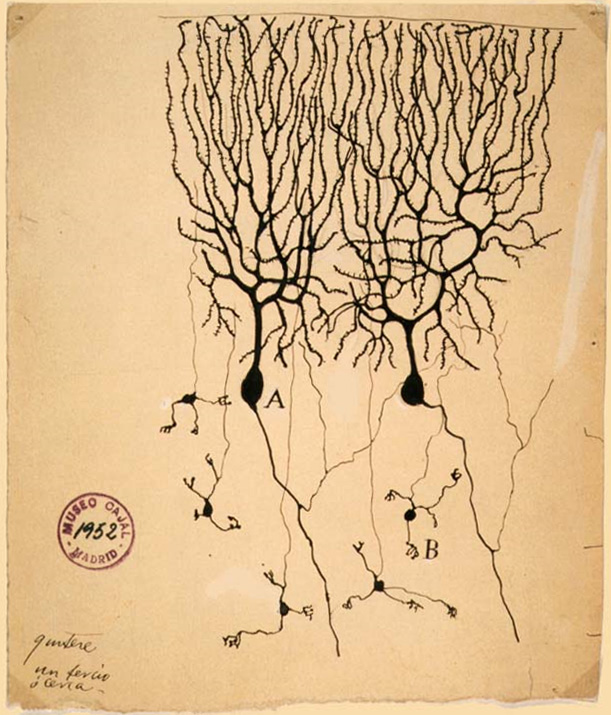
\includegraphics[width=0.30\linewidth]{images/book5/cajal-purkinje.jpg}\hspace{0.04\linewidth}
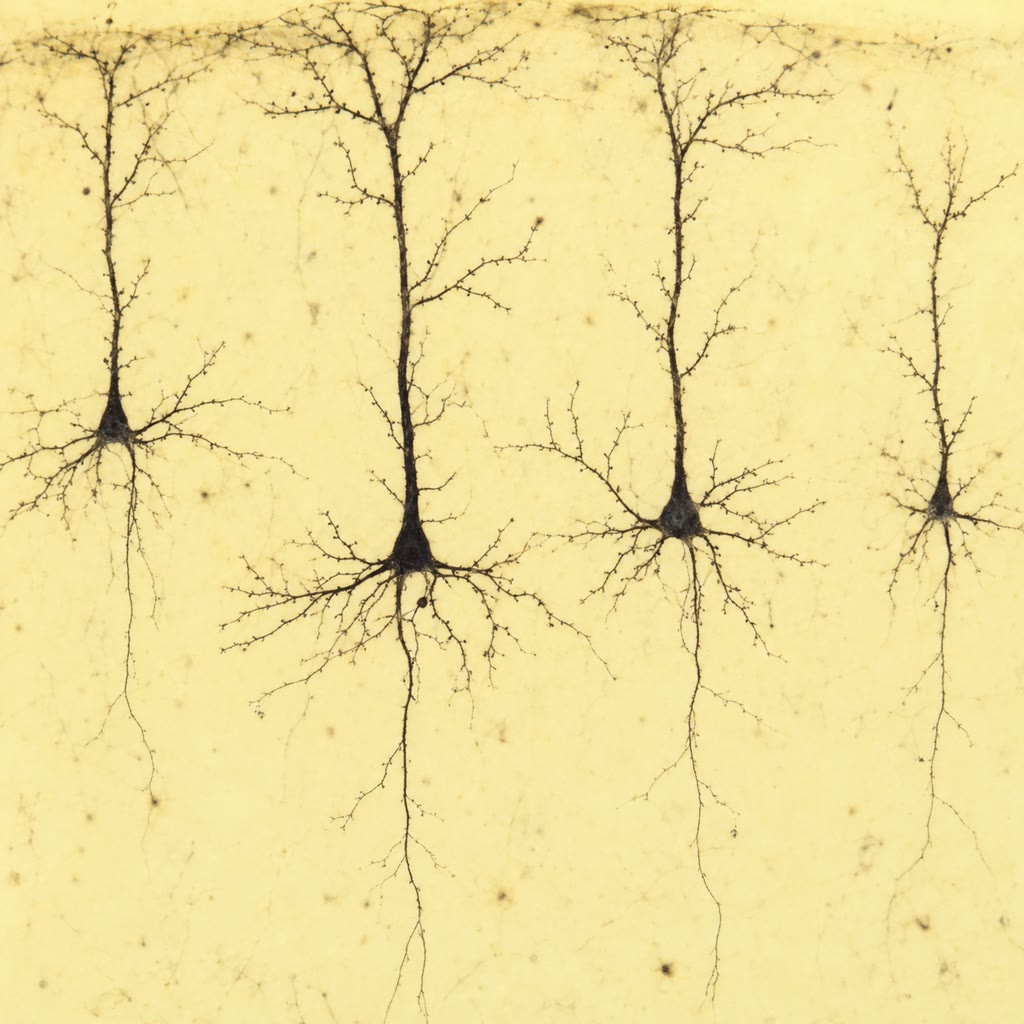
\includegraphics[width=0.30\linewidth]{images/book5/ai/b5-17-cortex-neurons.jpg}\hspace{0.04\linewidth}
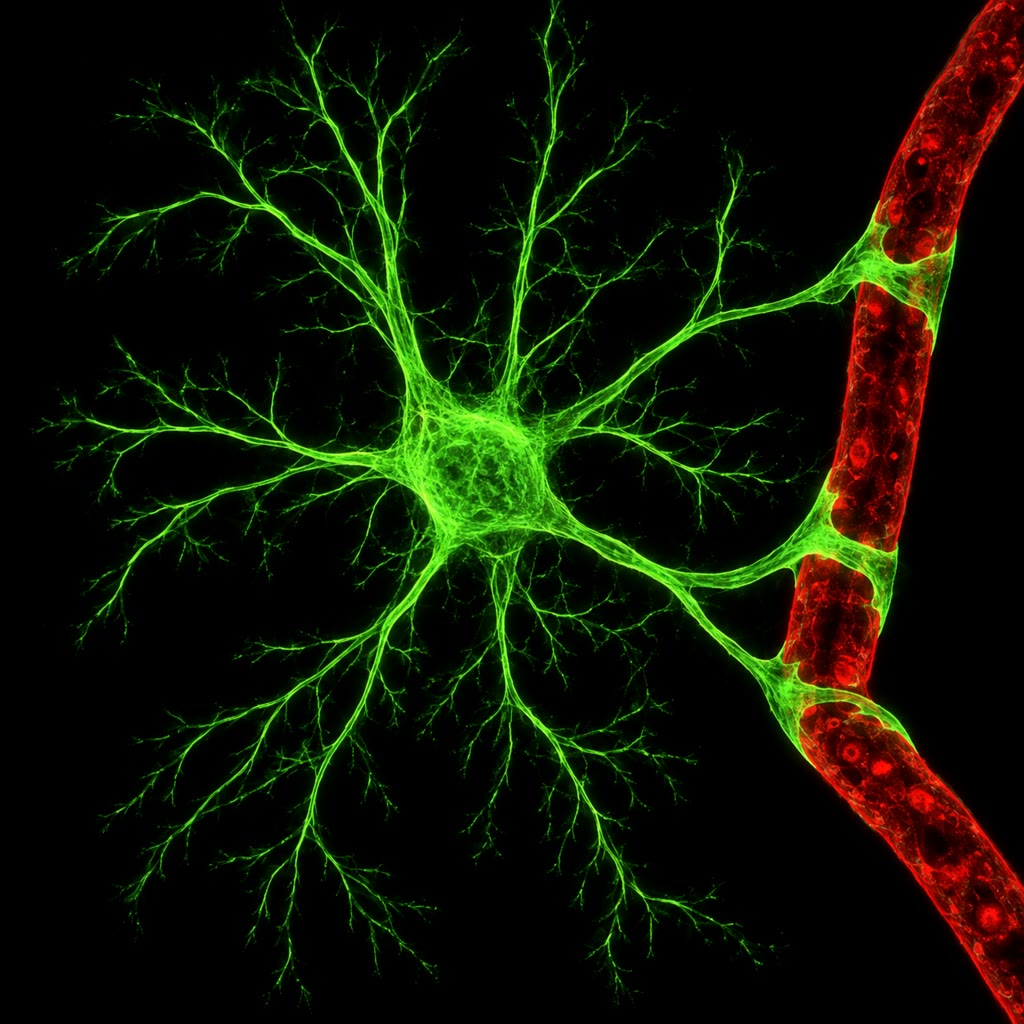
\includegraphics[width=0.30\linewidth]{images/book5/ai/b5-17-astrocyte.jpg}

{\small 左：卡哈尔（1899 年）绘制的\omterm{def:b3:nervous-systems:plan}{小脑}浦肯野细胞，
取自高尔基染色切片——整个单细胞的树突树，
是神经元作为独立单位的论据（公有领域）。中：
皮层的锥体神经元（高尔基染色）。右：一个\omterm{def:b3:nervous-systems:cells}{星形胶质细胞}
（绿色）及其终足附着于毛细血管（红色）上。}
\end{omfigure}

\section{神经元作为电缆}

\begin{theorem}[稳态电缆方程]\label{thm:b3:nervous-systems:cable}
\index{电缆方程}\index{长度常数}\index{时间常数!膜}\index{传导速度}
将树突或无髓轴突建模为直径为 $d$ 的圆柱体，
其胞质电阻率为 $R_{i}$，膜的比电阻为
$R_{m}$（电阻与面积之积）和单位
面积的电容 $C_{m}$。单位长度的轴向电阻为 $r_{i} = 4R_{i}/\pi d^{2}$，
而膜电阻为 $r_{m} = R_{m}/\pi d$。一个稳定电压
$V_{0}$ 施加于 $x = 0$ 处，沿纤维扩散为
\[
V(x) = V_{0}\,e^{-x/\lambda}, \qquad
\lambda = \sqrt{\frac{r_{m}}{r_{i}}} = \sqrt{\frac{R_{m}\,d}{4R_{i}}},
\]
其中 $\lambda$ 称为\emph{\omterm{thm:b3:nervous-systems:cable}{长度常数}}，指被动信号
衰减到 $1/e$ 所经过的距离，它随直径的平方根
增大。膜以\emph{时间常数} $\tau =
R_{m}C_{m}$ 充电，与几何形状无关。动作电位可自我再生，
沿无髓轴突传播，其速度
正比于 $\lambda/\tau$，因而正比于 $\sqrt{d}$；沿
有髓轴突中，动作电位在节点间跳跃，速度
正比于 $d$——约为每微米直径 \qty{6}{m/s}。
\end{theorem}
\begin{proof}
设 $I(x)$ 为轴向电流。沿轴心的欧姆定律给出
$\mathrm{d}V/\mathrm{d}x = -r_{i}I$；稳态下的电荷守恒表明，
在 $x$ 与 $x + \mathrm{d}x$ 之间损失的轴向电流
经膜漏出，即 $\mathrm{d}I/\mathrm{d}x = -V/r_{m}$。
对第一式求导并代入第二式，得
$\mathrm{d}^{2}V/\mathrm{d}x^{2} = (r_{i}/r_{m})V = V/\lambda^{2}$，这是一个
线性二阶方程，其在 $x \to \infty$ 时有界的解为
$V_{0}e^{-x/\lambda}$。将 $r_{m} = R_{m}/\pi d$ 与 $r_{i} =
4R_{i}/\pi d^{2}$ 代入，得 $\lambda^{2} = R_{m}d/4R_{i}$。时间常数为并联电阻与电容器的
乘积，$r_{m}c_{m} =
(R_{m}/\pi d)(C_{m}\pi d) = R_{m}C_{m}$。关于速度，
再生波须在约一个时间常数内，使膜充电至前方一个\omterm{thm:b3:nervous-systems:cable}{长度常数}处，
故 $v \sim \lambda/\tau \propto \sqrt{d}$；
在有髓轴突的节点之间，节间膜的
电阻升高、电容降低，二者皆源于一百多层
\omterm{def:b3:nervous-systems:cells}{髓鞘}，节间长度与 $d$ 成比例，结果为
$v \propto d$。比例常数在本阶段不加证明地承认。
\end{proof}

\begin{example}[一个树突与两根轴突的数值]\label{ex:b3:nervous-systems:numbers}
直径 $d = \qty{2}{\micro m}$ 的树突，其 $R_{m} = \qty{2e4}{\ohm.cm^2}$
及 $R_{i} = \qty{100}{\ohm.cm}$：$\lambda = \sqrt{2\times 10^{4}\times
2\times 10^{-4}/400}\ \unit{cm} = \qty{0.1}{cm} = \qty{1}{mm}$——一段毫米长的
树突末端的突触电位，到达
胞体时只剩其大小的三分之一，这正是树突树的几何形态
构成其运算的一部分。$\tau = 2\times 10^{4}\times
10^{-6}\,\unit{F/cm^2}\cdot\unit{\ohm.cm^2} = \qty{20}{ms}$，即输入须在
此时间窗内到达才能叠加。一根乌贼巨轴突，直径为
\qty{500}{\micro m}，无\omterm{def:b3:nervous-systems:cells}{髓鞘}，\omterm{thm:b3:nervous-systems:cable}{传导速度}约为 \qty{25}{m/s}；要达到同样的效果，
脊椎动物则用一根直径为 \qty{4}{\micro m} 的有髓轴突，
横截面积却小了一万五千倍——这正是
脊椎动物的神经能在一根乌贼巨轴突的空间里容纳
一万根快纤维的原因。一根 \qty{20}{\micro m} 的运动轴突，\omterm{thm:b3:nervous-systems:cable}{传导速度}为
\qty{120}{m/s}；多发性硬化症使其\omterm{def:b3:nervous-systems:cells}{髓鞘}脱落时，速度
降为原来的十分之一，并且在裸露段落处，传导可能完全中断。
\end{example}

\begin{omfigure}
\begin{tikzpicture}
\begin{axis}[
  width=6.4cm, height=5.2cm,
  axis x line=bottom, axis y line=left,
  xmin=0, xmax=3, ymin=0, ymax=1.05,
  xlabel={距离 (mm)}, ylabel={$V/V_{0}$},
  xlabel style={font=\small, at={(axis description cs:0.5,-0.12)}, anchor=north}, ylabel style={font=\small},
  tick label style={font=\scriptsize}, xtick={0,1,2,3}, ytick={0,0.37,1}, yticklabels={0,$1/e$,1},
  clip=false,
]
\addplot[very thick, omDef, domain=0:3, samples=60] {exp(-x/1.0)};
\addplot[very thick, omThm, domain=0:3, samples=60] {exp(-x/0.5)};
\node[font=\scriptsize, omDef, anchor=south west] at (axis cs:1.2,0.45) {$d = \qty{2}{\micro m}$，$\lambda = \qty{1}{mm}$};
\node[font=\scriptsize, omThm, anchor=north west] at (axis cs:0.8,0.22) {$d = \qty{0.5}{\micro m}$，$\lambda = \qty{0.5}{mm}$};
\end{axis}
\begin{axis}[
  at={(7.6cm,0)}, anchor=south west,
  width=6.4cm, height=5.2cm,
  xmode=log, ymode=log,
  xmin=0.1, xmax=1000, ymin=0.1, ymax=200,
  xlabel={轴突直径 ($\unit{\micro m}$)}, ylabel={速度 (m/s)},
  xlabel style={font=\small, at={(axis description cs:0.5,-0.12)}, anchor=north}, ylabel style={font=\small},
  tick label style={font=\scriptsize},
  clip=false,
]
\addplot[very thick, omDef, domain=1:25, samples=2] {6*x};
\addplot[very thick, omThm, domain=0.2:1000, samples=2] {1.1*sqrt(x)};
\fill[omThm] (axis cs:500,25) circle (2pt); \node[font=\scriptsize, anchor=north east] at (axis cs:500,23) {乌贼巨轴突};
\fill[omDef] (axis cs:20,120) circle (2pt); \node[font=\scriptsize, anchor=west] at (axis cs:26,120) {人类运动轴突};
\node[font=\scriptsize, omDef, anchor=north west, align=left] at (axis cs:1.2,60) {有髓：$v \propto d$};
\node[font=\scriptsize, omThm, anchor=north west, align=left] at (axis cs:2,0.7) {无髓：$v \propto \sqrt{d}$};
\end{axis}
\end{tikzpicture}

{\small 左：沿树突的稳态信号被动衰减，取两种直径——
\omterm{thm:b3:nervous-systems:cable}{长度常数}随 $\sqrt{d}$ 增大。右：\omterm{thm:b3:nervous-systems:cable}{传导速度}随直径的变化；\omterm{def:b3:nervous-systems:cells}{髓鞘}使
直径为 \qty{4}{\micro m} 的纤维，做到无髓轴突
需半毫米才能做到的事。}
\end{omfigure}

\section{回路}

\begin{definition}[基本回路]\label{def:b3:nervous-systems:circuits}
\index{反射弧}\index{交互抑制}\index{前馈抑制}\index{反馈抑制}\index{汇聚}\index{发散}
\emph{反射弧}是从感受器到效应器的最短通路：
在膝跳反射中，肌梭传入纤维进入\omterm{def:b3:nervous-systems:plan}{脊髓}，
并直接与同一肌肉的运动神经元形成突触，这些神经元
在叩击后约 \qty{30}{ms} 使该肌收缩——仅一个突触，无需大脑参与。
同一传入纤维还兴奋一个抑制性\omterm{def:b3:nervous-systems:cells}{中间神经元}，后者作用于
对侧肌肉的运动神经元（\emph{交互抑制}），使伸肌
的收缩不致被屈肌拮抗。多数回路
由少数\omterm{def:b3:bioinformatics:motif}{基序}构成：\emph{发散}，即一个神经元驱动
许多神经元，以及\emph{汇聚}，许多汇于一个，汇总证据；
\emph{前馈抑制}：一个输入同时兴奋靶神经元
和一个\omterm{def:b3:nervous-systems:cells}{中间神经元}，后者一毫秒后抑制靶神经元，
使反应在时间上更为锐利；\emph{反馈抑制}：
靶神经元自身的输出兴奋一个\omterm{def:b3:nervous-systems:cells}{中间神经元}，后者抑制它，
限制放电；若扩散至邻近神经元，则产生
侧向抑制，使对比度更为锐利（见\cref{ch:b3:sensory-systems}）；以及
\emph{去抑制}，即抑制一个抑制性神经元，是基底\omterm{def:b3:nervous-systems:comparative}{神经节}
释放运动的方式。
\end{definition}

\begin{omfigure}
\begin{tikzpicture}[every node/.style={font=\scriptsize}, >=stealth]
  % spinal cord cross-section (schematic)
  \draw[thick, omDef!60, fill=omDef!8] (5.4,1.5) ellipse (2.0 and 1.5);
  \draw[thick, gray, fill=gray!15] (5.4,1.5) .. controls (4.7,2.4) and (4.0,2.6) .. (4.0,1.9) .. controls (4.0,1.2) and (4.6,0.9) .. (4.8,0.5) .. controls (5.0,0.2) and (5.8,0.2) .. (6.0,0.5) .. controls (6.2,0.9) and (6.8,1.2) .. (6.8,1.9) .. controls (6.8,2.6) and (6.1,2.4) .. (5.4,1.5);
  \node[above] at (5.4,3.05) {脊髓};
  % muscles
  \draw[thick, omMeth!70!black, fill=omMeth!20] (0.2,0.2) rectangle (1.4,2.0); \node[below, align=center] at (0.8,0.1) {伸肌 \\（股四头肌）};
  \draw[thick, omThm!70!black, fill=omThm!15] (0.2,-2.6) rectangle (1.4,-1.4); \node[below, align=center] at (0.8,-2.7) {屈肌 \\（股后肌群）};
  \fill[omProp] (0.8,1.3) ellipse (0.12 and 0.3); \node[left, font=\tiny] at (0.65,1.3) {肌梭};
  % Ia afferent to cord (dorsal)
  \draw[very thick, omProp] (0.9,1.3) .. controls (2.0,2.6) and (3.6,2.9) .. (4.8,2.2); \fill[omProp] (4.8,2.2) circle (0.09);
  \node[above, omProp] at (2.6,2.85) {Ia 传入：牵张};
  % motor neuron to extensor
  \fill[omMeth!70!black] (5.0,0.9) circle (0.16);
  \draw[->, very thick, omMeth!70!black] (4.9,0.85) .. controls (3.4,0.3) and (2.0,0.4) .. (1.4,1.0);
  \draw[->, thick, omProp] (4.8,2.2) -- (5.0,1.1);
  % inhibitory interneuron to flexor motor neuron
  \fill[omThm] (6.1,1.7) circle (0.13);
  \draw[->, thick, omProp] (4.9,2.25) -- (6.0,1.8);
  \fill[omThm!70!black] (6.0,0.6) circle (0.16);
  \draw[-|, thick, omThm] (6.1,1.55) -- (6.0,0.8);
  \draw[->, very thick, omThm!70!black, dashed] (5.9,0.5) .. controls (4.8,-0.8) and (3.0,-1.6) .. (1.4,-2.0);
  % right-hand labels with leaders
  \node[right, omThm, font=\tiny] at (7.6,1.9) {Ia 类抑制性中间神经元}; \draw[gray, thin] (7.55,1.9) -- (6.25,1.7);
  \node[right, omMeth!70!black, font=\tiny, align=left] at (7.6,1.1) {伸肌运动神经元：兴奋}; \draw[gray, thin] (7.55,1.1) -- (5.15,0.9);
  \node[right, omThm!70!black, font=\tiny, align=left] at (7.6,0.3) {屈肌运动神经元：抑制}; \draw[gray, thin] (7.55,0.3) -- (6.15,0.6);
  \node[below] at (4.6,-0.15) {单突触反射：$\sim$\qty{30}{ms}};
  \node[below, align=center] at (4.2,-2.0) {交互抑制：\\拮抗肌舒张};
\end{tikzpicture}

{\small 牵张反射。叩击拉伸伸肌的肌梭；
Ia 类传入纤维直接兴奋伸肌运动神经元（一
个突触），并经一个抑制性\omterm{def:b3:nervous-systems:cells}{中间神经元}抑制屈肌的运动神经元。}
\end{omfigure}

\begin{proposition}[中枢模式发生器]\label{prop:b3:nervous-systems:cpg}
\index{中枢模式发生器}\index{半中枢振荡器}
节律性运动——呼吸、行走、游泳、咀嚼——
由\omterm{def:b3:nervous-systems:plan}{脑干}和\omterm{def:b3:nervous-systems:plan}{脊髓}中能够自行振荡的回路产生，
这些回路即\emph{\omterm{prop:b3:nervous-systems:cpg}{中枢模式发生器}}，感觉反馈可以调节其活动，
但不能产生它们：一只猫的\omterm{def:b3:nervous-systems:plan}{脊髓}在与脑分离并切断感觉神经后，
仍能产生交替的
迈步模式。最简单的设计是布朗的\emph{半中枢}（1911）：
两群神经元各自抑制对方。哪一组先放电，
就会抑制另一组；但放电的一组会疲劳——其通道失活，
对伙伴的抑制随之减弱——而伙伴，
解除抑制后开始放电，继而抑制先前的一组：形成交替，其周期
由疲劳的时间常数决定，而非任何时钟。
呼吸节律产生于延髓中由数千个神经元组成的一簇
神经元（pre-Bötzinger 复合体），自出生起即以爆发形式放电，
直到死亡；七鳃鳗的游泳由沿\omterm{def:b3:nervous-systems:plan}{脊髓}排列的一串半中枢构成，
每一个都比前一个延迟激活，使波动向尾部传播。
\end{proposition}

\begin{omfigure}
\begin{tikzpicture}[every node/.style={font=\scriptsize}, >=stealth]
  % half-centre
  \begin{scope}
    \draw[thick, fill=omDef!25] (0,0) circle (0.5); \node at (0,0) {左};
    \draw[thick, fill=omThm!25] (3,0) circle (0.5); \node at (3,0) {右};
    \draw[-|, very thick] (0.5,0.2) -- (2.5,0.2); \draw[-|, very thick] (2.5,-0.2) -- (0.5,-0.2);
    \node[above] at (1.5,0.3) {相互抑制};
    \draw[->, thick, omDef] (0,-0.5) -- (0,-1.3) node[below] {左侧肌肉};
    \draw[->, thick, omThm] (3,-0.5) -- (3,-1.3) node[below] {右侧肌肉};
    \draw[->, thick, gray] (-1.2,0.6) -- (-0.45,0.25) node[pos=0, above, align=center] {来自脑干的 \\紧张性驱动};
    \draw[->, thick, gray] (4.5,0.6) -- (3.45,0.25);
  \end{scope}
  % traces
  \begin{scope}[xshift=6.0cm, yshift=0.9cm]
    \node[left, omDef] at (0,0) {左};
    \foreach \x in {0,2,4} { \foreach \s in {0.1,0.2,...,0.9} \draw[omDef] (\x+\s,-0.15) -- (\x+\s,0.15); }
    \node[left, omThm] at (0,-1.0) {右};
    \foreach \x in {1,3,5} { \foreach \s in {0.1,0.2,...,0.9} \draw[omThm] (\x+\s,-1.15) -- (\x+\s,-0.85); }
    \draw[->] (0,-1.6) -- (6.2,-1.6) node[right] {时间};
    \draw[<->] (0,-2.0) -- (2,-2.0) node[midway, below] {周期：由疲劳决定};
  \end{scope}
\end{tikzpicture}

{\small \omterm{prop:b3:nervous-systems:cpg}{半中枢振荡器}。两组相互抑制的神经元在
持续驱动下交替放电：活跃一侧疲劳，其抑制
减弱，另一侧脱离抑制并接替放电。单个神经元本身
并不具有节律性。}
\end{omfigure}

\begin{method}[追踪神经回路]\label{met:b3:nervous-systems:tracing}
\index{神经回路追踪}\index{光遗传学}
要确定神经元 A 驱动神经元 B，且该通路
对某一行为有影响：（1）解剖学——注入沿轴突运输的示踪剂
（染料，或一种改造狂犬\omterm{def:b3:virology:virus}{病毒}，可逆向跨越一个突触
），找出相连的细胞；（2）生理学——在记录 B 的同时
刺激 A，并测量潜伏期（单突触连接
给出约一毫秒的固定延迟），以及性质（兴奋或
抑制）；（3）必要性——使 A 沉默，可通过损毁、降温，或
在 A 中表达光驱动氯泵并照光
（\emph{\omterm{met:b3:nervous-systems:tracing}{光遗传学}}），观察行为是否失效；（4）
充分性——单独激活 A，用光驱动阳离子通道，
观察行为是否出现；（5）在完整动物中，
用钙指示剂对神经元群体的活动成像，同时
行为进行时的活动。五项结果一致时，回路即告确立；
已发表的多数回路只有两三个环节。
\end{method}

\section{脊椎动物神经系统的总体结构}

\begin{definition}[中枢与外周部分]\label{def:b3:nervous-systems:plan}
\index{脊髓}\index{脑干}\index{小脑}\index{丘脑}\index{下丘脑}\index{大脑皮层}\index{自主神经系统}\index{肠神经系统}
\emph{中枢神经系统}即脑与脊髓；
其余部分为\emph{外周}。\emph{脊髓}经背根接收
感觉轴突，经腹根发出运动轴突，
其灰质呈细胞体组成的蝶形，其
白质则是上下走行的有髓纤维束。
\emph{脑干}——延髓、脑桥、中脑——包含
脑神经核，以及无需意识参与即可维持呼吸、心率和
血压的中枢；脑干死亡即意味着死亡。
\emph{小脑}神经元数量多于脑的其余部分，负责调节
运动的时序与协调，并能从误差中学习。
\emph{丘脑}将除嗅觉外的所有感觉传递至皮层，
并将皮层的反馈送回；位于其下方的\emph{下丘脑}
主管稳态——体温、饥饿、口渴、生物钟、内分泌
轴（见\cref{ch:b3:endocrinology}）。\emph{基底\omterm{def:b3:nervous-systems:comparative}{神经节}}负责从
可能的动作中进行选择；\emph{海马}形成记忆
（见\cref{ch:b3:learning-memory}）；而\emph{大脑皮层}是一片
由六层细胞构成的薄片，厚两至四毫米，面积为四分之一
平方米，折叠以适应颅腔，承担其余功能，其中
为各种感觉和运动定位的区域，以及它们之间的联络区。
外周系统的\emph{自主神经}部分支配各器官：\emph{交感}
神经链释放去甲肾上腺素，使机体动员（心跳加快，
胃肠活动减弱，瞳孔放大）；\emph{副交感}神经释放
乙酰胆碱，使机体保存能量并促进消化；而\emph{肠}
神经系统由肠壁中的五亿个神经元构成，
独立支配消化。
\end{definition}

\begin{omfigure}
\begin{tikzpicture}[every node/.style={font=\scriptsize}, >=stealth]
  % sagittal brain schematic
  \draw[thick, omDef!70, fill=omDef!15] (0,2.0) .. controls (0,4.6) and (3.5,5.4) .. (6.0,4.4) .. controls (7.6,3.7) and (7.4,2.2) .. (6.2,1.9) .. controls (5.4,1.7) and (5.2,1.3) .. (4.4,1.6) .. controls (3.0,1.3) and (1.2,1.4) .. (0,2.0);
  \node[align=center] at (3.0,3.9) {大脑皮层：六层，\\感觉、运动与联络区};
  % basal ganglia / hippocampus (deep)
  \draw[thick, omProp!70, fill=omProp!25] (3.2,2.6) ellipse (0.9 and 0.45); \node[font=\tiny] at (3.2,2.6) {基底神经节};
  \draw[thick, omProp!70, fill=omProp!25] (5.2,2.45) ellipse (0.88 and 0.3); \node[font=\tiny] at (5.2,2.45) {海马};
  % thalamus, hypothalamus
  \draw[thick, omMeth!70!black, fill=omMeth!25] (4.0,1.95) ellipse (0.7 and 0.3); \node[font=\tiny] at (4.0,1.95) {丘脑};
  \draw[thick, omMeth!70!black, fill=omMeth!40] (4.0,1.42) ellipse (0.78 and 0.22); \node[font=\tiny] at (4.0,1.42) {下丘脑};
  % cerebellum
  \draw[thick, omThm!70, fill=omThm!20] (6.6,1.2) ellipse (0.9 and 0.6); \node[font=\tiny] at (6.6,1.2) {小脑};
  % brainstem
  \draw[thick, gray!70, fill=gray!20] (4.7,1.2) -- (5.5,1.2) -- (5.9,-0.3) -- (5.1,-0.3) -- cycle; \node[font=\tiny, rotate=-75] at (5.3,0.45) {脑干};
  % spinal cord
  \draw[thick, gray!70, fill=gray!20] (5.2,-0.3) rectangle (5.8,-1.6); \node[right, font=\tiny] at (5.85,-1.0) {脊髓};
  % labels with leaders on the right
  \node[right, align=left] at (7.8,3.4) {丘脑：传递除嗅觉外的 \\各种感觉；下丘脑：\\稳态、生物钟、内分泌轴};
  \draw[gray] (7.75,3.3) -- (4.7,1.95);
  \node[right, align=left] at (7.8,1.9) {小脑：调节时序与 \\协调，从误差中学习};
  \draw[gray] (7.75,1.8) -- (7.5,1.4);
  \node[right, align=left] at (7.8,0.4) {脑干：呼吸、心跳、\\脑神经（延髓、\\脑桥、中脑）};
  \draw[gray] (7.75,0.4) -- (5.9,0.4);
  \node[right, align=left] at (7.8,-1.0) {脊髓：反射、模式发生器、\\上下走行的纤维束};
\end{tikzpicture}

{\small 矢状面中的脊椎动物脑（示意）：皮层
覆盖在深部核团之上，\omterm{def:b3:nervous-systems:plan}{丘脑}与\omterm{def:b3:nervous-systems:plan}{下丘脑}居中，
\omterm{def:b3:nervous-systems:plan}{小脑}位于后方，\omterm{def:b3:nervous-systems:plan}{脑干}向下延续为\omterm{def:b3:nervous-systems:plan}{脊髓}。}
\end{omfigure}

\begin{proposition}[血脑屏障与脑的能量预算]\label{prop:b3:nervous-systems:barrier-budget}
\index{血脑屏障}\index{脑脊液}\index{脑能量预算}
脑的毛细血管内皮细胞之间以紧密连接封闭，
外面包裹着\omterm{def:b3:nervous-systems:cells}{星形胶质细胞}的足突，并配有转运蛋白，
允许葡萄糖和氨基酸通过，并将其他许多物质泵出，
这一结构即\emph{\omterm{prop:b3:nervous-systems:barrier-budget}{血脑屏障}}，它维持脑细胞外液的离子组成恒定，
以保证神经元的电学行为，
并排除大多数药物，
（\qty{98}{\%}的小分子和全部\omterm{def:b3:adaptive-immunity:antibody}{抗体}）——神经药理学的核心难题。
脑漂浮于 \qty{150}{mL} 的
\emph{\omterm{prop:b3:nervous-systems:barrier-budget}{脑脊液}}中，以每分钟半毫升的速度生成，每天更新四次，
起缓冲作用，并带走废物，尤以睡眠期间为甚。
脑的耗能：成年人约为 \qty{20}{W}，
占静息代谢的 \qty{20}{\%}，几乎全部来自葡萄糖氧化生成 ATP，
其中大部分 ATP 被钠泵消耗，用以恢复
动作电位和突触电流不断耗散的梯度。按每摩尔 ATP
\qty{50}{kJ} 计算，\qty{20}{W} 相当于每秒 $4\times 10^{-4}$ mol
的 ATP，即 $2.4\times 10^{20}$ 个分子。
平均分配到 $8.6\times 10^{10}$ 个神经元上，每个神经元每秒约 $3\times 10^{9}$ 个 ATP。
一次皮层动作电位及其突触后果
的耗能约为 $10^{9}$ 个 ATP 的量级，因此预算只允许
每个神经元平均每秒发放几个脉冲，
而皮层神经元确实大致以此频率发放。脑是按严格的能量上限设计的，
这正是其信号稀疏、轴突纤细、
信息由许多细胞中的少量脉冲编码的原因。
\end{proposition}
\admitted

\section{各类动物的神经系统}

\begin{definition}[神经网、神经节与脑]\label{def:b3:nervous-systems:comparative}
\index{神经网}\index{神经节}\index{头部集中化}\index{脑化}
刺胞动物（如水母、Hydra）具有\emph{神经网}：神经元
分布于体壁中，向各个方向相互连接，并在
伞缘周围形成环状聚集结构，协调
游泳运动——没有中心，沿每个细胞的传导
可以双向进行。两侧对称动物将神经元集中为\emph{神经节}——
共享神经毡的细胞群——沿腹侧神经索排列，
见于节肢动物和环节动物，其头部神经节在感觉
器官集中处增大，即\emph{头部集中化}。软体动物从河蚌的简单神经节
到章鱼不等，章鱼的神经元约五亿个，是所有无脊椎动物中最多的，
其中三分之二位于腕中，每条腕各自
的神经索控制自身的伸展与抓取。脊椎动物则发育出
背侧中空神经管，前端扩展为上一节所述的脑，
并受骨骼与\omterm{def:b3:innate-immunity:innate}{屏障}保护，且具有\omterm{def:b3:nervous-systems:cells}{髓鞘}。
相同的信号分子、离子通道、神经递质
以及许多相同的发育基因（后脑的 Hox 密码、眼部图式因子），
支配着所有这些类型：各部件古老且共有，
而其排布方式则多种多样。
\end{definition}

\begin{example}[神经元计数]\label{ex:b3:nervous-systems:counts}
线虫有 $302$ 个神经元，每一个都有名字，每个突触都已绘制；
果蝇 $1.4\times 10^{5}$ 个；蜜蜂 $10^{6}$ 个；小鼠
$7\times 10^{7}$ 个；章鱼 $5\times 10^{8}$ 个；人类 $8.6\times
10^{10}$ 个；大象 $2.6\times 10^{11}$ 个，其中大部分位于
\omterm{def:b3:nervous-systems:plan}{小脑}。跨哺乳动物，脑质量与体质量大致按
$M_{\text{脑}} \propto M_{\text{体}}^{0.75}$ 的关系变化，因此小鼠的脑
在体重中所占比例比大象更大；物种若高于
同体型直线之上——如海豚、灵长类，人类高出
约七倍——则被称为\omterm{def:b3:nervous-systems:comparative}{脑化}。与认知能力关系最密切的
不是脑质量，而是\omterm{def:b3:nervous-systems:plan}{大脑皮层}中神经元的数目：人类约
$1.6\times 10^{10}$ 个，大象为 $5.6\times 10^{9}$ 个，其脑
体积约为人类的三倍；黑猩猩为 $2\times 10^{9}$ 个。人类
大脑在细胞与构造上并无特殊之处；
但皮层神经元数目比任何其他物种都多，排布也更密集，
而起作用的似乎是数目，而非重量。
\end{example}

\begin{omfigure}
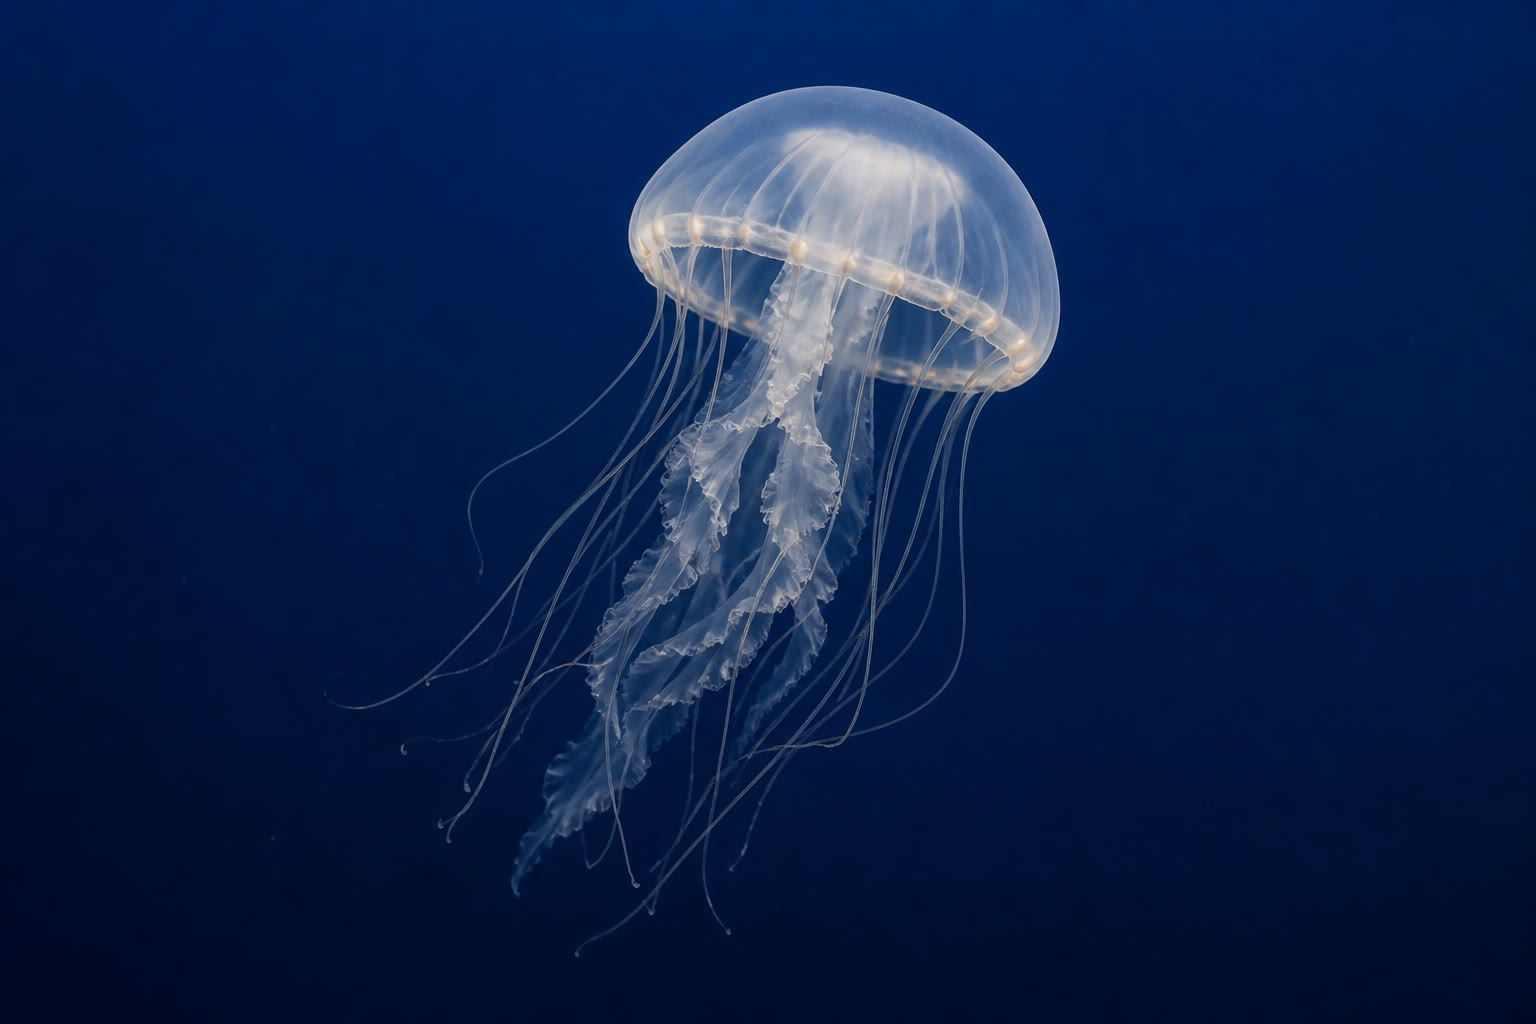
\includegraphics[width=0.46\linewidth]{images/book5/ai/b5-17-jellyfish.jpg}\hspace{0.04\linewidth}
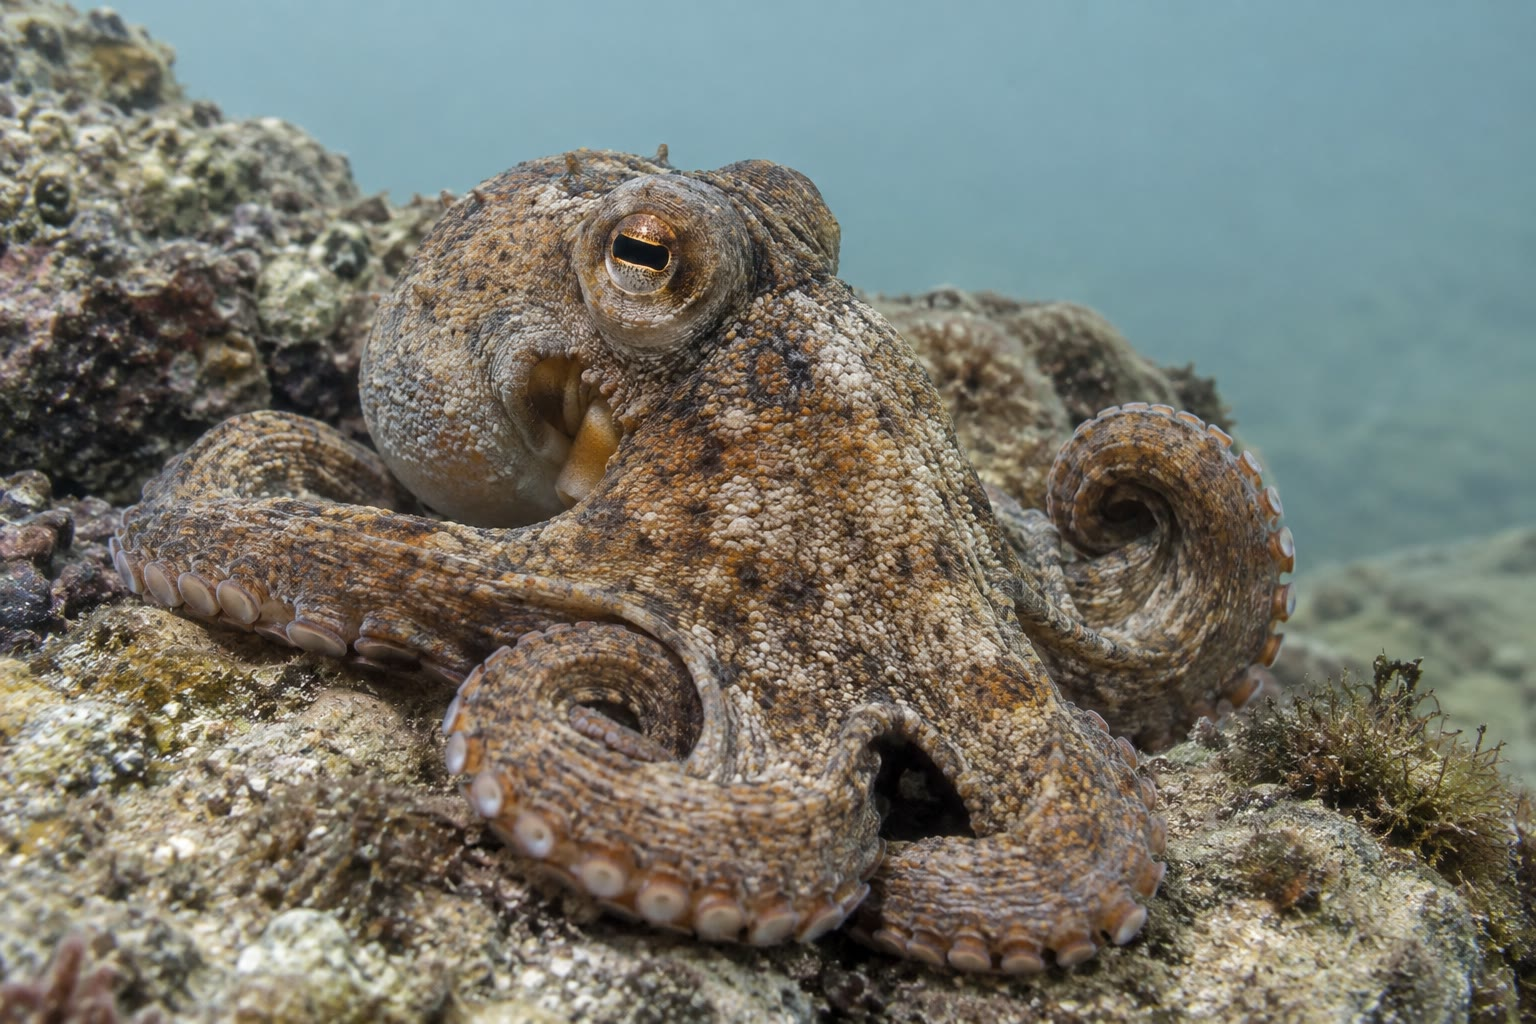
\includegraphics[width=0.46\linewidth]{images/book5/ai/b5-17-octopus.jpg}

{\small 神经元的两种组织方式。左：水母，其\omterm{def:b3:nervous-systems:comparative}{神经网}
与伞缘环状结构协调游泳，却没有脑。右：
章鱼拥有五亿个神经元，大部分位于腕中，并
具有所有无脊椎动物中最大的脑。}
\end{omfigure}

\begin{remark}[神经系统的作用]\label{rem:b3:nervous-systems:for}
植物、真菌和海绵都没有神经系统；能够运动的动物则需要神经系统，
神经系统的复杂化程度与运动、远距离感知，
以及预测接下来将发生之事的需求相适应。
\omterm{thm:b3:nervous-systems:cable}{电缆方程}规定了物理上的限制——信号能传多远、多快，
取决于给定的直径与绝缘情况；能量预算决定了经济上的约束；
在这些限制之内，同样的神经元以网状、\omterm{def:b3:nervous-systems:comparative}{神经节}
或皮层的方式排布，便产生了水母的脉冲、章鱼的伪装，
或此刻这句话。接下来两章讨论输入端
与存储：感觉如何把世界转化为脉冲，以及
突触如何发生改变，使得世界一经遇到便被记住。
\end{remark}

\section{练习}

\begin{exercise}[$\star$]\label{exo:b3:nervous-systems:1}
说出\omterm{def:b3:nervous-systems:cells}{神经胶质}的四种类型及各自的一项功能，并说明
哪两种产生\omterm{def:b3:nervous-systems:cells}{髓鞘}，以及它们位于何处。
\end{exercise}

\begin{exercise}[$\star$]\label{exo:b3:nervous-systems:2}
高尔基染色法使何种研究成为可能？卡哈尔据此得出了什么结论，
高尔基又得出了什么结论？哪一方正确，又是如何裁定的？
\end{exercise}

\begin{exercise}[$\star$]\label{exo:b3:nervous-systems:3}
描述膝跳\omterm{def:b3:nervous-systems:circuits}{反射弧}，并解释为何它只需
\qty{30}{ms}，而随意踢腿所需时间长十倍。
\end{exercise}

\begin{exercise}[$\star$]\label{exo:b3:nervous-systems:4}
列出交感神经和副交感神经对心脏、
瞳孔、肠道和气道的作用，以及每一类神经在靶器官处所用的
递质。
\end{exercise}

\begin{exercise}[$\star\star$]\label{exo:b3:nervous-systems:5}
计算直径为 \qty{1}{\micro m} 的轴突的\omterm{thm:b3:nervous-systems:cable}{长度常数}，其中 $R_{m}
= \qty{1e4}{\ohm.cm^2}$，$R_{i} = \qty{100}{\ohm.cm}$，并求经过
\qty{2}{mm} 后信号剩余的比例。若要使 $\lambda$ 加倍，
直径应为多少？
\end{exercise}

\begin{exercise}[$\star\star$]\label{exo:b3:nervous-systems:6}
一根直径为 \qty{12}{\micro m} 的感觉轴突从脚趾延伸 \qty{1.2}{m}
到\omterm{def:b3:nervous-systems:plan}{脊髓}，一根直径为 \qty{15}{\micro m} 的运动轴突再由\omterm{def:b3:nervous-systems:plan}{脊髓}返回。
取 \qty{6}{m/s} 每微米的速度和 \qty{0.5}{ms} 每个突触的延迟，估算
含一个\omterm{def:b3:nervous-systems:cells}{中间神经元}的\omterm{def:b3:nervous-systems:plan}{脊髓}撤回反射的最短潜伏期。
若改用同直径的无\omterm{def:b3:nervous-systems:cells}{髓鞘}轴突，取
$v = 1.1\sqrt{d}$，则需多长时间？
\end{exercise}

\begin{exercise}[$\star\star$]\label{exo:b3:nervous-systems:7}
利用
\cref{prop:b3:nervous-systems:barrier-budget}中的大\omterm{prop:b3:nervous-systems:barrier-budget}{脑能量预算}，估算一个
神经元每秒可消耗多少 ATP，若一个动作电位及其突触的耗能为
$2\times 10^{9}$ 个 ATP，求该预算允许的平均放电频率。这对
编码有何预测？
\end{exercise}

\begin{exercise}[$\star\star$]\label{exo:b3:nervous-systems:8}
解释\omterm{prop:b3:nervous-systems:cpg}{半中枢振荡器}为何需要疲劳（或其他慢过程）才能振荡，
并说明若两个相互抑制的神经元
永不疲劳，会出现什么情况。
\end{exercise}

\begin{exercise}[$\star\star$]\label{exo:b3:nervous-systems:9}
\omterm{prop:b3:nervous-systems:barrier-budget}{血脑屏障}阻止 L-多巴的产物多巴胺通过，却允许
L-多巴通过。解释这一性质如何用于帕金森病的治疗，以及为何
针对脑蛋白的\omterm{def:b3:adaptive-immunity:antibody}{抗体}难以递送。
\end{exercise}

\begin{exercise}[$\star\star\star$]\label{exo:b3:nervous-systems:10}
推导\omterm{thm:b3:nervous-systems:cable}{电缆方程}的含时形式 $\lambda^{2}\,\partial^{2}
V/\partial x^{2} = \tau\,\partial V/\partial t + V$，通过将电容电流与膜电流相加，
并证明定理的稳态解由此成立。
（只需写出该形式，无需求解。）
为什么比值 $\lambda/\tau$ 是一个速度？
\end{exercise}

\begin{exercise}[$\star\star\star$]\label{exo:b3:nervous-systems:11}
鱿鱼巨轴突直径为 \qty{500}{\micro m}，\omterm{thm:b3:nervous-systems:cable}{传导速度}为 \qty{25}{m/s}。
利用 $v \propto \sqrt{d}$，无\omterm{def:b3:nervous-systems:cells}{髓鞘}轴突要达到
\qty{100}{m/s} 的速度需要多大直径？计算其横截面积，并与
达到同一速度的直径为 \qty{20}{\micro m} 的有\omterm{def:b3:nervous-systems:cells}{髓鞘}轴突进行比较。这说明
一根神经所能承载的快肌纤维数量有何限制，以及
对\omterm{def:b3:nervous-systems:cells}{髓鞘}的演化意味着什么？
\end{exercise}

\begin{exercise}[$\star\star\star$]\label{exo:b3:nervous-systems:12}
跨哺乳动物而言，脑质量与 $M_{\text{体重}}^{0.75}$ 成比例。
一只 \qty{30}{g} 的小家鼠脑重 \qty{0.4}{g}。预测一只
\qty{70}{kg} 哺乳动物的脑质量，沿此标度关系估算，与人类的 \qty{1350}{g} 比较，并讨论为何
皮层神经元数目而非脑质量，
是认知能力更好的相关指标。
\end{exercise}

\section{问题：身体的布线}

\begin{problem}[{周末问题——以长度常数、毫秒和瓦特计算身体的布线：一个树突与两根轴突的电缆参数，
从脚趾到脊髓再返回的反射潜伏期，大脑为每个动作电位所能承担的能量，
以及不同动物脑的标度关系，最后
求长度常数、反射潜伏期，
以及大脑能够支付的
平均放电频率}]
\label{pb:b3:nervous-systems:1}
数据：$R_{m} = \qty{2e4}{\ohm.cm^2}$，$R_{i} = \qty{100}{\ohm.cm}$，
$C_{m} = \qty{1}{\micro F/cm^2}$。有\omterm{def:b3:nervous-systems:cells}{髓鞘}轴突的速度为 \qty{6}{m/s} 每微米；
无\omterm{def:b3:nervous-systems:cells}{髓鞘}轴突 $v = 1.1\sqrt{d}$ m/s，其中 $d$ 以微米计；
突触延迟为 \qty{0.5}{ms}。大脑：功率 \qty{20}{W}，
$8.6\times 10^{10}$ 个神经元，$10^{14}$ 个突触，ATP 为 \qty{50}{kJ/mol}；
一个动作电位耗能 $4\times 10^{8}$ 个 ATP，每次突触传递耗能 $2\times 10^{4}$ 个 ATP；
一个神经元有 \num{7000} 个突触。标度关系：
$M_{\text{脑}} = a\,M_{\text{体重}}^{0.75}$，其中一只 \qty{30}{g} 的小家鼠
脑重 \qty{0.4}{g}。

\medskip
\noindent\textbf{第一部分——电缆。}
\begin{enumerate}
  \item 计算直径为 \qty{1}{\micro m} 与
        \qty{4}{\micro m} 的树突的 $\lambda$，以及 $\tau$。
  \item 位于 \qty{1}{\micro m} 树突上、距胞体 \qty{300}{\micro m} 处的突触
        局部产生 \qty{5}{mV} 的电位。到达胞体的电位为多少？
        在 \qty{4}{\micro m} 的树突上，又为多少？
  \item 解释为何神经元能够依据输入落在树突树上
        的位置对其加权，以及为何输入必须在
        约 $\tau$ 的时间内到达才能求和。
  \item 计算直径为 \qty{10}{\micro m} 的有\omterm{def:b3:nervous-systems:cells}{髓鞘}轴突的速度，
        以及同直径无\omterm{def:b3:nervous-systems:cells}{髓鞘}轴突的速度。要使无\omterm{def:b3:nervous-systems:cells}{髓鞘}轴突的速度与有\omterm{def:b3:nervous-systems:cells}{髓鞘}轴突相同，
        其直径应为多少？
  \item 计算 \qty{10}{\micro m} 轴突与等效无\omterm{def:b3:nervous-systems:cells}{髓鞘}轴突的
        横截面积。在一根等效无\omterm{def:b3:nervous-systems:cells}{髓鞘}轴突所占的空间内，
        可容纳多少根有\omterm{def:b3:nervous-systems:cells}{髓鞘}轴突？
  \item 某脱\omterm{def:b3:nervous-systems:cells}{髓鞘}疾病使一根直径为
        \qty{10}{\micro m} 的轴突在 \qty{2}{cm} 的长度上失去\omterm{def:b3:nervous-systems:cells}{髓鞘}。估算若该段
        按同直径的无\omterm{def:b3:nervous-systems:cells}{髓鞘}轴突传导时的额外延迟，
        并说明传导为何可能完全失效。
\end{enumerate}

\medskip
\noindent\textbf{第二部分——潜伏期。}
\begin{enumerate}[resume]
  \item 脚趾接触到热的表面。感觉轴突（\qty{10}{\micro m}，
        \qty{1.2}{m}）到达\omterm{def:b3:nervous-systems:plan}{脊髓}，经过一个\omterm{def:b3:nervous-systems:cells}{中间神经元}，再由运动轴突
        （\qty{15}{\micro m}，\qty{1.1}{m}）返回腿部。撤回反射的最短
        潜伏期为多少？
  \item 信号还沿直径为 \qty{10}{\micro m} 的轴突
        传过 \qty{0.6}{m} 到达大脑，并再经过两个突触，之后才感到疼痛。
        相对于撤回反射，何时感到疼痛？
  \item 一根疼痛纤维无\omterm{def:b3:nervous-systems:cells}{髓鞘}，直径为 \qty{1}{\micro m}。其信号
        沿 \qty{1.8}{m} 传到大脑需要多长时间？
        解释踢到脚趾时疼痛的两个阶段。
  \item 一只长颈鹿的腿比上述的腿还长 \qty{2}{m}。重新计算反射潜伏期，
        并评论体型大小带来的问题。
  \item 膝跳反射是单突触的，成人中为 \qty{30}{ms}。取往返各
        \qty{0.8}{m}、速度为 \qty{80}{m/s}，计入一个突触和一个神经肌肉接头
        （\qty{1}{ms}），以及肌肉产生力所需的 \qty{5}{ms}，
        解释这 \qty{30}{ms} 的构成。
  \item 新生儿的轴突无\omterm{def:b3:nervous-systems:cells}{髓鞘}。解释其反射为何缓慢、
        动作为何不协调，以及
        出生后前两年的\omterm{def:b3:nervous-systems:cells}{髓鞘}形成改变了什么。
\end{enumerate}

\medskip
\noindent\textbf{第三部分——能量预算。}
\begin{enumerate}[resume]
  \item 将 \qty{20}{W} 换算为每秒生成的 ATP 数，
        以及每个神经元每秒生成的 ATP 数。
  \item 一个神经元发放一次脉冲：其自身耗用 $4\times 10^{8}$ 个 ATP，
        并驱动 \num{7000} 个突触，每个突触耗用 $2\times 10^{4}$ 个 ATP。
        一次脉冲连同其后果的总耗能是多少？
  \item 若全部预算都用于脉冲发放，预算能维持的
        平均发放率是多少？若其中一半用于静息消耗呢？
  \item 皮层神经元的平均发放频率约为 \qty{1}{Hz}。这占预算的
        多大比例，它说明了什么，
        关于信息的编码方式？
  \item 若每个神经元都以 \qty{50}{Hz} 发放，需要多少
        瓦特？与全身的 \qty{100}{W} 相比如何？
  \item 葡萄糖以 \qty{5}{g/h} 的速率供给大脑。这相当于
        多少瓦特（取 \qty{16}{kJ/g}）？是否足够，
        以及供应中断后数秒之内，意识会发生什么？
\end{enumerate}

\medskip
\noindent\textbf{第四部分——尺度关系。}
\begin{enumerate}[resume]
  \item 由小鼠数据求出 $a$，再预测一只 \qty{70}{kg} 哺乳动物
        和一头 \qty{5000}{kg} 大象的脑质量，
        均由该直线给出。
  \item 实际值：人类 \qty{1350}{g}，大象 \qty{4800}{g}。分别计算
        各物种的实际值与预测值之比
        （即\omterm{def:b3:nervous-systems:comparative}{脑化}商）。
  \item 大象的脑有 $2.6\times 10^{11}$ 个神经元，皮层中却只有
        $5.6\times 10^{9}$ 个；人类则分别为 $8.6\times 10^{10}$
        和 $1.6\times 10^{10}$。大象的神经元位于何处？这说明皮层的
        功能是什么？
  \item 神经元的体积随轴突长度增加而增大，因此较大的脑
        拥有更大、更稀疏的神经元。解释为何脑质量加倍后
        神经元数目并不随之加倍，以及灵长类的神经元在脑增大时
        保持较小，因而每克脑组织中的神经元数
        多于啮齿类动物。
  \item 章鱼有 $5\times 10^{8}$ 个神经元，其中三分之二位于
        腕中。请提出在没有脑的情况下，一条腕能做什么、不能做什么，
        并设计一个实验来检验这一设想。
  \item 线虫 \emph{C.~elegans} 有 $302$ 个神经元，
        突触总数约为 \num{7000}，且每个都已被绘出。比较它每个神经元的
        突触数与人类的数值，并说明一张完整的连线图
        能够告诉我们哪些关于行为的信息，又有哪些不能。
  \item 综合以下三个量：\qty{1}{\micro m} 树突的\omterm{thm:b3:nervous-systems:cable}{长度常数}
        （第 1 题）、退缩反射的潜伏期（第 7 题），
        以及在一半能量用于脉冲时，脑的能量预算所允许的平均发放频率
        （第 15 题）。
\end{enumerate}
\end{problem}
